% Intra-shard vs. cross-shard (2PC) transaction, ported from the SOAPS paper
\tikzset{
  shard/.style={draw=gray!50, rounded corners=5pt, fill=gray!5},
  committee/.style={draw=gray!30, rounded corners=3pt, fill=gray!6},
  statepart/.style={draw=gray!30, rounded corners=3pt, fill=orange!4},
  vnode/.style={draw=gray!60, fill=gray!25, circle, minimum size=0.38cm, inner sep=0pt},
  acct/.style={draw=gray!40, fill=white, rounded corners=1pt, font=\tiny,
               minimum width=1.0cm, minimum height=0.27cm, inner sep=1pt},
  beacon/.style={draw=gray!40, fill=gray!8, rounded corners=4pt},
  parthead/.style={draw=gray!45, fill=gray!10, rounded corners=2pt, font=\scriptsize, inner sep=3pt},
  lifeline/.style={gray!30, thin},
  intratx/.style={->, >=stealth, thick, green!60!black},
  cstx/.style={->, >=stealth, thick, orange!70!black},
  cstxr/.style={->, >=stealth, thick, orange!60!black, dashed},
}

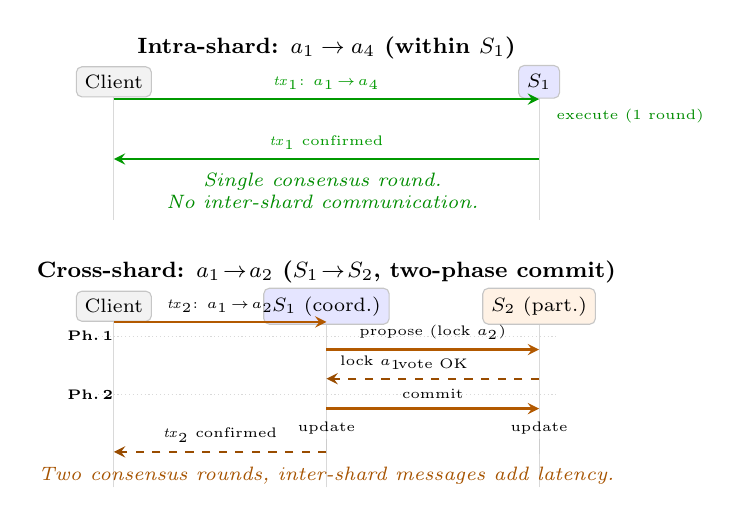
\begin{tikzpicture}[>=stealth]

\node[font=\footnotesize\bfseries] at (3.50,3.53)
  {Intra-shard: $a_1 \to a_4$ (within $S_1$)};

% Lifelines
\draw[lifeline] (0.8,1.35) -- (0.8,3.05);
\draw[lifeline] (6.2,1.35) -- (6.2,3.05);

% Participant headers
\node[parthead] at (0.8,3.10) {Client};
\node[parthead, fill=blue!10] at (6.2,3.10) {$S_1$};

% (1) Submit
\draw[intratx] (0.8,2.88) -- (6.2,2.88);
\node[font=\tiny, above, green!60!black] at (3.50,2.88)
  {$\mathit{tx}_1$: $a_1\!\to\!a_4$};

\node[font=\tiny, right, green!55!black] at (6.3,2.66) {execute (1 round)};

% (2) Confirmed
\draw[intratx] (6.2,2.12) -- (0.8,2.12);
\node[font=\tiny, above, green!60!black] at (3.50,2.12)
  {$\mathit{tx}_1$ confirmed};

% Summary
\node[font=\scriptsize, green!55!black, align=center] at (3.45,1.72)
  {\textit{Single consensus round.}\\
   \textit{No inter-shard communication.}};

%%──────────────────────────────────────────────────────────────────────────────
%% BOTTOM: Cross-shard 2PC transaction
%%──────────────────────────────────────────────────────────────────────────────
\begin{scope}[yshift=-2.85cm]

\node[font=\footnotesize\bfseries, align=center] at (3.50,3.53)
  {Cross-shard: $a_1\!\to\!a_2$ ($S_1\!\to\!S_2$, two-phase commit)};

% Lifelines
\draw[lifeline] (0.80,0.80) -- (0.80,3.05);
\draw[lifeline] (3.50,0.80) -- (3.50,3.05);
\draw[lifeline] (6.20,0.80) -- (6.20,3.05);

% Participant headers
\node[parthead]                 at (0.80,3.10) {Client};
\node[parthead, fill=blue!10]   at (3.50,3.10) {$S_1$ (coord.)};
\node[parthead, fill=orange!10] at (6.20,3.10) {$S_2$ (part.)};

% (1) Submit
\draw[cstx] (0.80,2.90) -- (3.50,2.90);
\node[font=\tiny, above] at (2.15,2.90)
  {$\mathit{tx}_2$: $a_1\!\to\!a_2$};

% Phase 1 separator
\draw[gray!30, densely dotted] (0.60,2.72) -- (6.45,2.72);
\node[font=\tiny\bfseries, black] at (0.50,2.72) {\textbf{Ph.\,1}};

% (2) Propose: S1 → S2
\draw[cstx] (3.50,2.55) -- (6.20,2.55);
\node[font=\tiny, above] at (4.85,2.55) {propose (lock $a_2$)};
\node[font=\tiny, right, black] at (3.55,2.38) {lock $a_1$};

% (3) Vote OK: S2 → S1
\draw[cstxr] (6.20,2.18) -- (3.50,2.18);
\node[font=\tiny, above] at (4.85,2.18) {vote OK};

% Phase 2 separator
\draw[gray!30, densely dotted] (0.60,1.98) -- (6.45,1.98);
\node[font=\tiny\bfseries, black] at (0.50,1.98) {\textbf{Ph.\,2}};

% (4) Commit: S1 → S2
\draw[cstx] (3.50,1.80) -- (6.20,1.80);
\node[font=\tiny, above] at (4.85,1.80) {commit};

% Update-state boxes
\draw[gray!40,thin] (3.50,1.42) -- (3.50,1.22);
\draw[gray!40,thin] (6.20,1.42) -- (6.20,1.22);
\node[font=\tiny, black, align=center] at (3.50,1.55) {update};
\node[font=\tiny, black, align=center] at (6.20,1.55) {update};

% (5) Confirmed
\draw[cstxr] (3.50,1.25) -- (0.80,1.25);
\node[font=\tiny, above] at (2.15,1.25) {$\mathit{tx}_2$ confirmed};

% Summary
\node[font=\scriptsize, orange!65!black, align=center] at (3.50,0.95)
  {\textit{Two consensus rounds, inter-shard messages add latency.}};

\end{scope}
\end{tikzpicture}
